\documentclass[dvipsnames]{standalone}

\usepackage[english]{babel}
\usepackage[linesnumbered, ruled, vlined]{algorithm2e}

\usepackage{caption}

% to create listings

\usepackage{listings, lstautogobble}
\lstset{
  autogobble=true,
  frame=single,
}

\lstdefinelanguage{coq}[Objective]{Caml}{
  morekeywords={Structure, Definition, Inductive, list, return},
  sensitive=true
}

% to define font size

\usepackage{ulem}
\usepackage{moresize}
\usepackage{anyfontsize}

% to use tikz and its libraries

\usepackage{tikz-timing}
\usepackage{tikz}
\usepackage{tikz-qtree}

\usetikzlibrary{backgrounds}
\usetikzlibrary{decorations.pathreplacing, positioning, calc, arrows, shapes, automata, petri, patterns}

% to use tikzmark, to place and refer to marks outside the current figure

% \tikzset{every picture/.style={remember picture}}

% styles for transitions

\tikzset{transition/.append style={fill=black!20, thick}}
\tikzset{transition/.append style={fill=black!20, thick}}

% styles for test and inhib arcs.

\tikzstyle{test}=[pre, *-]
\tikzstyle{inhib}=[pre, o-]

% to use colors

\usepackage{xcolor}

%%%%%%%%%%%%%%%%%%%%%%%%%%%%%%%%%%%%%%%%%%%%%%%%%%
%                  BEGIN DOCUMENT                %
%%%%%%%%%%%%%%%%%%%%%%%%%%%%%%%%%%%%%%%%%%%%%%%%%%

\begin{document}

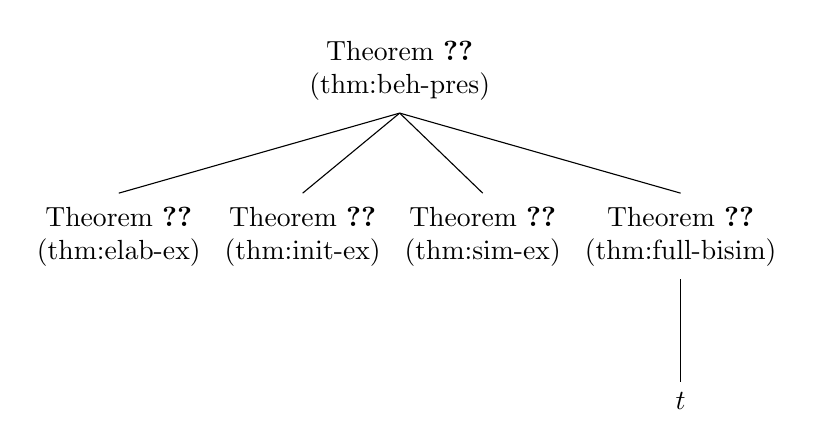
\begin{tikzpicture}
  \tikzset{level distance=60pt}
  \Tree [.\node {
      \begin{tabular}{@{}c@{}}
        Theorem~\ref{thm:beh-pres} \\
        (\nameref{thm:beh-pres}) \\
      \end{tabular}
    };
    [.\node {
      \begin{tabular}{@{}c@{}}
        Theorem~\ref{thm:elab-ex} \\
        (\nameref{thm:elab-ex}) \\
      \end{tabular}
    }; ]
    [.\node {
      \begin{tabular}{@{}c@{}}
        Theorem~\ref{thm:init-ex} \\
        (\nameref{thm:init-ex}) \\
      \end{tabular}
    }; ]
    [.\node {
      \begin{tabular}{@{}c@{}}
        Theorem~\ref{thm:sim-ex} \\
        (\nameref{thm:sim-ex}) \\
      \end{tabular}
    }; ]
    [.\node {
      \begin{tabular}{@{}c@{}}
        Theorem~\ref{thm:full-bisim} \\
        (\nameref{thm:full-bisim}) \\
      \end{tabular}
    }; \node {$t$}; ]
  ]
  
  % \Tree [.Theorem

    %   
  %   [.Theorem z % \node {
  %   %   \begin{tabular}{@{}c@{}}
  %   %     Theorem~\ref{thm:elab-ex} \\
  %   %     (\nameref{thm:elab-ex}) \\
  %   %   \end{tabular}
  %   % };
  %   ]
  %   [.Theorem a ]
  %   [.Theorem b ]
  %   [.Theorem c ] ]
   
  
\end{tikzpicture}

\end{document}